\documentclass{article}
\usepackage{listings}
\usepackage{graphicx}
% \usepackage[utf8]{inputenc}
% \usepackage[T1]{fontenc}
\title{Algoritmi Bread-First and Depth-First su Adjacency Matrix and Adjacency List Graphs}
\author{Patrick Jusic}


\usepackage{color}

\definecolor{mGreen}{rgb}{0,0.6,0}
\definecolor{mGray}{rgb}{0.5,0.5,0.5}
\definecolor{mPurple}{rgb}{0.58,0,0.82}
\definecolor{backgroundColour}{rgb}{0.95,0.95,0.92}

\lstdefinestyle{CStyle}{
    backgroundcolor=\color{backgroundColour},
    basicstyle=\footnotesize,
    commentstyle=\color{mGreen},
    keywordstyle=\color{magenta},
    numberstyle=\tiny\color{mGray},
    stringstyle=\color{mPurple},
    basicstyle=\footnotesize,
    breakatwhitespace=false,
    breaklines=true,
    captionpos=b,
    keepspaces=true,
    numbers=left,
    numbersep=5pt,
    showspaces=false,
    showstringspaces=false,
    showtabs=false,
    tabsize=2,
    language=C++
}


\begin{document}
\maketitle{}
\paragraph{}
\paragraph{}
\paragraph{}

% \begin{figure}
  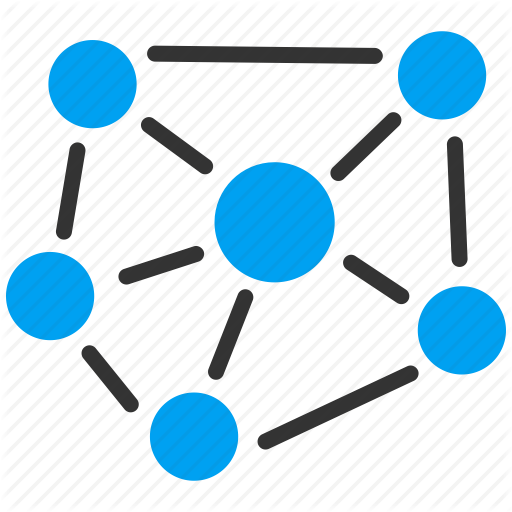
\includegraphics[width=\linewidth]{graph.png}
  % \caption{A Graph.}
  % \label{fig:graph1}
% \end{figure}


\pagenumbering{gobble}
\newpage
\tableofcontents
\newpage
\pagenumbering{arabic}

\section{Progetto}
\subsection{Introduzione}
L'argomento del progetto \`e l'implementazione di grafi con le tecniche di \textit{Adjacency Matrix} e \textit{Adjacency Lists}, e l'impego di queste classi in algoritmi di esplorazione della frontiera. \newline
L'obbiettivo \`e stato il confronto delle prestazioni dei due tipi di grafo, sia a livello strutturale, sia a livello implementativo degli stessi algoritmi. \newline
Un appunto iniziale che vorrei fare \`e specificare che questo progetto \`e stato sviluppato durante il corso, a cavallo tra lo studio degli alberi e delle tabelle hash, cos\`i da intendere che alcune mancanze o affermazioni imprecise potrebbero essere motivate dall'impreparazione su argomenti, come ad esempio i tipi di dato astratto, che non sono ancora stati trattati. \newline
Con questa premessa, prima di entrare nella descrizione delle parti implementate, vorrei sottolineare ci\`o che mi ha pi\`u colpito nella trattazione dei grafi, cio\`e l' elevato grado di astrazione che caratterizza l'implementazione di questa struttura. \newline
Infatti se inizialmente pu\`o venir naturale pensare ad un implementazione simile a quella seguita negli alberi, risulta poi molto pi\`u semplice a livello di sviluppo e concettuale, aumentare il grado di astrazione e gestire questa struttura con una struttura pi\`u semplice, come ad esempio una matrice, che non fa uso di puntatori. Questa tecnica risulta, infatti, implementativamente pi\`u semplice rispetto a quella mediante l'uso di liste. \newline
Nel progetto non \`e stata trattata l'implementazione di algoritmi per la ricerca di un elemento, classici dell'argomento, che si basano sull'ottimizzazione della ricerca attraverso il percorso pi\`u breve possibile. Qui si apre una finestra molto ampia che meriterebbe un intero progetto al riguardo e qualche altro centinaio di righe di codice per poterne affrontare tutti gli aspetti.\newline
Entrambe le classi implementate sono corredate di metodi che le rendono utilizzabili non solo nella suddetta applicazione, ma gi\`a pronte ad essere incorporate con nuovi metodi per diverse applicazioni. Sono implementati metodi per l'aggiunta di collegamenti tra i nodi, la loro rimozione, il controllo e la stampa. Non \`e stata prevista la possibilit\`a di mettere un limite al numero dei nodi e dei loro collegamento.


\subsection{Adjacency Matrix}
L' implementazione con la matrice di adiacenza si basa come precedentemente sottolineato sulla creazione di una matrice rappresentante il grafo, associandone i nodi agli indici di righe e colonne. \newline
Il parametro di creazione della matrice \`e \texttt{vertexCount} che rappresenta il numero di nodi del grafo. Viene quindi generata una matrice vuota di $vertexCount^2$ elementi, ognuno settato a \textrm{0}. \newline
Successivamente, tramite i metodi implementati nella classe, si procede alla creazione degli \texttt{Edges}, i collegamenti tra i grafi, rappresentati con il numero \textrm{1}. Quindi, in corrispondenza dell'indice riga \textit{i-esimo} e dell'indice colonna \textit{j-esimo}, si trova l'\textrm{1} che rappresenta il collegamento tra il nodo \textit{i-esimo} e il nodo \textit{j-esimo} del grafo. \newline
Questo \`e un collegamento \texttt{Diretto}, caratteristica che pu\`o caratterizzare l'intero grafo, e significa che l'edge originato dal nodo \textit{i-esimo} con destinazione il nodo \textit{j-esimo}, non pu\`o essere percorso in senso opposto. In questo caso si parlerebbe di collegamento \texttt{Indiretto}, che risulterebbe in un \textrm{1} nella matrice in corrispondenza tra l'indice della riga \textit{j-esima} e l'indice della colonna \textit{i-esima}. Intuitivamente risulta che se il grafo \`e completamente \texttt{Indiretto} \`e rappresentato da una matrice simmetrica. \newline
L'uso di \textrm{1} e \textrm{0} \`e molto utile per rappresentare la presenza di un grafo, ma pu\`o essere rimpiazzato con l'utilizzo di valori $\epsilon [0,1]$, cos\`i da rappresentare un grafo con collegamenti pesati, utile in applicazioni come ad esempio reti neurali. \newline

\subsection{Adjacency List}
L' implementazione con lista di adiacenza ricorda maggiormente il tipo di struttura ad albero perch\`e presenta in modo esplicito delle struct \texttt{Node}, ognuno dei quali contiene il valore corrispondente all'indice del nodo rappresentato, ed un puntatore all'elemento successivo.\newline
L'idea \`e quella di rappresentare un array di puntatori, della lunghezza di \texttt{vertexCount}, il quale riferisce all'indice dell'elemento \textit{i-esimo} il nodo \textit{i-esimo} del grafo, elemento dal quale parte il puntatore ad una lista contenente tutti i nodi della frontiera del nodo \textit{i-esimo}. La frontiera \`e l'insieme dei nodi collegati al nodo in questione. Tale struttura pu\`o ricordare idealmente quella del vettore di bucket discusso nella Tabelle Hash.\newline
Quindi la generazione del grafo si compone della creazione dell'array, e dell'inizializzazione a NULL di tutti i suoi puntatori. Successivamente con un metodo della classe si aggiungono elementi alla lista corrispondente, anche qui con il principio di collegamento \texttt{Diretto} o \texttt{Indiretto}.
Risulta evidente la maggior complessit\`a di sviluppo di questa struttura, ma in realt\`a l'implementazione dei metodi ad essa relativi non risultano poi particolarmente ostici.

\subsection{Algoritmi}
L'idea dietro gli algoritmi implementati \`e quella di esplorare il grafo, attraverso due differenti approcci.\newline
Per poter tener traccia dell'esplorazione si concettualizza con la colorazione dei nodi il loro stato. La dichiarazione di tale concetto \`e svolta attraverso l'\textit{enum} \texttt{VertexState},  che elenca i tre diversi stati possibili cio\`e:
\begin{itemize}
  \item \texttt{White}: questo stato descrive il nodo come mai visitato
  \item \texttt{Grey}: questo stato descrive il nodo in fase di esplorazione, cio\`e quando la sua frontiera \`e in fase di esplorazione
  \item \texttt{Black}: questo stato descrive il nodo in post-esplorazione, quando cio\`e tutta la sua frontiera \`e stata esplorata
\end{itemize}
L'algoritmo di esplorazione si dir\`a concluso quando tutti i nodi del grafo saranno stati colorati di nero, ad eccezione di quei nodi che non sono collegati a nessun altro nodo e non hanno modo di essere raggiunti, i quali risuleranno inesistenti per il grafo.\newline
La complessit\`a computazionale di entrambi gli algoritmi \`e \textit{$\theta(n)$}, dato che in entrambi i casi il grafo viene completamente esplorato, quindi bisogner\`a visitare tutti gli \textit{n} nodi presenti nella sua struttura.

\subsubsection{Depth-First Algorithm}
L'algoritmo Depth-First \`e costruito in modo tale da inseguire la profondit\`a del grafo. Come dice il nome infatti questo algoritmo esplora il grafo puntando al fondo di esso, esplorando via via ogni nodo mancante. \newline
Perci\`o verr\`a passato come parametro \texttt{start}, cio\`e il nodo da cui cominciare. Una volta messo il suo stato a grigio con un \textit{for} si comincia ad esplorare la sua frontiera. Ricorsivamente lo stesso procedimento verr\`a applicata al primo nodo incontrato nella frontiera del nodo inziale, che verr\`a anch'esso messo a grigio. \newline
Il nodo iniziale viene colorato di nero soltanto quando tutta la sua frontiera sar\`a esplorata, perci\`o quando tutti i suoi figli, e quindi i figli dei suoi figli, e cos\`i via, saranno gi\`a stati esplorati.\newline
Quindi l'approccio di questo algoritmo \`e quello di esplorare il grafo seguendo la sua lunghezza puntando sempre alle foglie, quei nodi cio\`e che non hanno figli.

\subsubsection{Breadth-First Algorithm}
L'algoritmo Breadth-First, a differenza del suo collega procede per gradi, esplorando man mano l'intera frontiera del nodo che in questa fase \`e colorato di grigio. \newline
Quindi come nel caso precedente, all'interno di un ciclo \textit{for}, tutti i nodi collegati al nodo in questione vengono colorati di grigio, ma differenza del Depth-First, lo stato del nodo la cui frontiera \`e stata completamente visitata \`e messo a nero, ben prima quindi che lo diventino i suoi figli, e i figli dei figli, i quali saranno successivamenti ricorsivamente sottoposti allo stesso processo.\newline
Perci\`o in questo caso le foglie sono raggiunte solamente quando tutti i figli del nodo di partenza sono gi\`a stati esplorati e colorati di nero.

\subsection{Confronto tra Algoritmi}
Intuitivamente il Breadth-First risulta pi\`u performante, specie per quanto riguarda la ricerca di un elemento. In realt\`a le performance dei due algoritmi sono profondamente condizionate dalla struttura del grafo, come verr\`a poi illustrato nella sezione \texttt{Risultati}.\newline
In particolare il Breadth-First pu\`o risultare inefficiente se i nodi cercati sono in fondo al grafo, le cosiddette foglie, mentre il discorso opposto vale per il Depth-First nel momento in cui il nodo cercato \`e l'ultimo dei figli del nodo iniziale, in quanto dev'essere esplorata prima gran parte del grafo.\newline
Per quanto riguarda la ricerca bisognerebbe perci\`o differenziare casi peggiori e casi migliori contemplando una complessit\`a computazionale che pu\`o andare da \textit{$\theta(1)$} fino a \textit{$\theta(n)$}, inversamente in base all'algoritmo applicato. \newline
Non avendo sviluppato il discorso di ricerca di un elemento questo discorso decade in parte, cio\`e che la struttura del grafo dovrebbe condizionare un po' meno il \textit{tempo effettivo di esecuzione}, avendo entrambi gli algoritmi complessit\`a computazionale \textit{$\theta(n)$}, ed essendo impiegati con lo stesso fine. In realt\`a ci sar\`a modo di esporre i risultati e discuterne il significato.

\newpage
\section{Codice}
Sono di seguito riportati tutti i codici che compongono il progetto suddivisi in base agli header files, cio\`e i files linkati, e il programma principale dove sono state svolte le prove. \newline
Nel programma principale \`e stata implementata la funzione \texttt{decorateGraph}, con lo scopo di generare in maniera randomica dei grafi, con entrambi i modi di sviluppo presentati, con lo stesso numeri di nodi e collegamenti, per avere dei confronti il pi\`u affidabili possibile.\newline
Oltre ai files header contenenti le classi che implementano i grafi, sono stati linkati altri due file, uno contenente una classe \texttt{Timer}, che sfrutta la libreria \texttt{ctime} per calcolare il tempo effettivo di esecuzione degli algoritmi in microsecondi, e l'altro contente l'implementazione di una \texttt{Queue}, con la struttura e metodi discussi durante il corso, utilizzata nel Breadth-First della Matrice di Adiacenza.

\subsection{Headers}
\subsubsection{Matrice di Adiacenza}
\lstinputlisting[style=CStyle]{"../AdjacencyMatrix.h"}
\subsubsection{Lista di Adiacenza}
\lstinputlisting[style=CStyle]{"../AdjacencyList.h"}
\subsubsection{Queue}
\lstinputlisting[style=CStyle]{"../Queue.h"}
\subsubsection{Timer}
\lstinputlisting[style=CStyle]{"../Timer.h"}
\subsection{Main}
\lstinputlisting[style=CStyle]{"../main.cpp"}

\newpage
\section{Risultati}
In questa sezione vengono riportati gli output del software sui quali svolgere le adeguate considerazioni e le analisi statistiche risultanti.\newline
Non sono sicuramente stati analizzati tutti i casi possibili, ma la speranza \`e che i dati portati permettano un'analisi pertinente del problema. \newline
Ci tengo a sottolineare che i tempi effettivi di esecuzione riportati possono essere condizionati da una mancata ottimizzazione degli algoritmi in questione, ragion per cui con una differente codifica potrebbero essere smentiti. In particolar l'utilizzo di una coda nel Breadth-First, sviluppato nella matrice di adiacenza, applicazione basata sulla letteratura esistente, mi suggerisce una possibile miglioria, rispetto agli altri algoritmi che non ne fanno uso e si risparmiano la generazione e la gestione di un'altra struttura dati che grava sul tempo effettivo di esecuzione.

\subsection{Output}
Sono stati riportati 5 esempi di output con un numero di nodi componenti la struttura crescente, scelti perch\`e sembrano portare spunti interessanti, analizzandone i tempi effettivi di esecuzioni. \newline
\subsubsection{5 Nodi}
In questa configurazione, con un basso numero di nodi ed un discreto numero percentuale di collegamenti tra di essi, in entrambe le implementazioni il Depth-First vanta quasi un ordine di grandezza inferiore relativo al suo tempo effettivo di esecuzione rispetto a quello del Breadth-First. \newline
I tempi del Depth-First sono molto vicini, mentre guadagna qualcosa il Breadth-First della lista di adiacenza implementato senza utilizzo di una coda.
\lstinputlisting[style=CStyle]{"../5nodes.txt"}
\subsubsection{9 Nodi}
Con 9 nodi si avvicinano i tempi degli algoritmi di esplorazione per la lista di adiacenza, mentre restano ancora lontani quelli per la matrice di adiacenza dove il Depth-First \`e ancora nettamente pi\`u rapido.
\lstinputlisting[style=CStyle]{"../9nodes.txt"}
\subsubsection{10 Nodi}
Con solamente un nodo in pi\`u i tempi di esecuzione si riducono ancora ma mantengono la stessa proporzione del grafo con 9 nodi.
\lstinputlisting[style=CStyle]{"../10nodes.txt"}
\subsubsection{14 Nodi}
Con 14 nodi si nota una stabilizzazione sui tempi di esecuzione, c'\`e un miglioramento del Breadth-First rispetto al Depth-First, per la lista di adiacenza, che fin qui era sempre stato pi\`u lento.
\lstinputlisting[style=CStyle]{"../14nodes.txt"}
\subsubsection{21 Nodi}
Con 21 nodi si conferma l'intuizione precedente perch\`e il Breadth-First si dimostra pi\`u veloce rispetto al Depth-First, sempre per quanto riguarda la lista di adiacenza.
\lstinputlisting[style=CStyle]{"../21nodes.txt"}

\subsection{Commenti}
L' efficienza degli algoritmi sembra esser influenzata molto da quella che \`e la grandezza del grafo, cio\`e il numero di nodi, e relativamente per quelli che sono i collegamenti tra di essi. \newline
Per configurazioni piccole il Depth-First supera addirittura l'ordine di grandezza dei microsecondi, raggiungendo i $10^-7$ secondi, mentre il Breadth-First soffre decisamente di pi\`u, specie nel caso della matrice di adiacenza, dove sembra essere decisivo l'utilizzo della coda.\newline
Aumentando il numero di nodi si nota che i tempi tendono a livellarsi e dalle prove svolte, una volta raggiunti i 50 nodi si raggiunge un punto di equilibrio tra i tempi di esecuzione di tutti gli algoritmi di esplorazione in cui nessuno riesce a toccare l'ordine di grandezza dei microsecondi per tempo effettivo di esecuzione. \newline
La prova con il maggior numero di nodi, 103, ha confermato questo equilibrio, mostrando un'aumentare proporzionale di tutti i tempi, tranne per quello del Breadth-First della lista di adiacenza, che a differenza degli altri algoritmi che esibiscono tempi dell'ordine di grandezza di $10^-4$, mantiene un $10^-5$, di poco superiore rispetto alle prove fatte con la met\`a dei nodi.\newline
Queste ultime prove mettono in luce la migliore efficienza del Breadth-First rispetto al Depth-First, descritta nella letteratura, quando ci si trova ad affrontare strutture dati di una certa portanza. \newline
Realisticamente il Depth-First che offre tempi migliori con piccole strutture non \`e poi confrontabile con il Breadth-First in quanto difficilmente algoritmi di ricerca saranno applicati su grafi della grandezza di 10 nodi.\newline
Il passo successivo \`e l'implementazione di algoritmi di ricerca come l'\textit{A*}, per avere un confronto reale su quella che \`e la complessit\`a computazionale dei due algoritmi e i loro tempi effettivi di esecuzione in un problema utilizzato in diversi ambiti quali database implementati con grafi, che rappresentano l'essenza di questo problema.

\end{document}
